\chapter{Regression + Classification}

\section*{Objective}
Classification models using a lot of predictors give a model which might be complex. The objective thus is to try to use a simple linear regression model to determine the least number of attributes which affect the class to be predicted and then construct classification models.
\\
\\
Here the marks of the students are used to predict the NRC{\_}CLASS variable using a classification model.

\section*{Procedure}
\begin{itemize}
\item Marks of all languages and subjects have already been discretized as in ~/ref{chap:experiment1}.
\item Typically a linear regression model with more number of predictors gives a better fitted model. Thus for every count of the number of courses, from 1 to 5(not including all the courses), the best combination of predictors are chosen.
\begin{itemize}
\item For a number $n$,the best combination of predictors are found building regression models for all possible combination of attributes and the standard deviation of their residuals.
\end{itemize}
\item From each of these best combination of predictors a classification model is built.
\begin{itemize}
\item The classification model chosen is KNN as the predictors are numeric attributes. $k$ was chosen to be 10 after manual inspection with several values.
\end{itemize}
\item The accuracy of each of these classification models is compared to find out the best classification model.
\end{itemize}

\section*{Observations}
\begin{itemize}
\item Best predictors obtained
\begin{lstlisting}
> best_models
[[1]] # For n = 1
lm(formula = TOTAL_MARKS ~ S2_MARKS)

[[2]] # For n = 2
lm(formula = TOTAL_MARKS ~ L1_MARKS + L2_MARKS)

[[3]] # For n = 3
lm(formula = TOTAL_MARKS ~ L1_MARKS + L2_MARKS + S3_MARKS)

[[4]] # For n = 4
lm(formula = TOTAL_MARKS ~ L1_MARKS + L2_MARKS + S1_MARKS + S3_MARKS)

[[5]] # For n = 5
lm(formula = TOTAL_MARKS ~ L1_MARKS + L2_MARKS + L3_MARKS + S1_MARKS 
                           + S3_MARKS)
\end{lstlisting}
\item Comparision of misclassification errors for different number of predictors(Best combination)
\begin{figure}[h!]
  %\caption{Decision Tree}
  \centering
    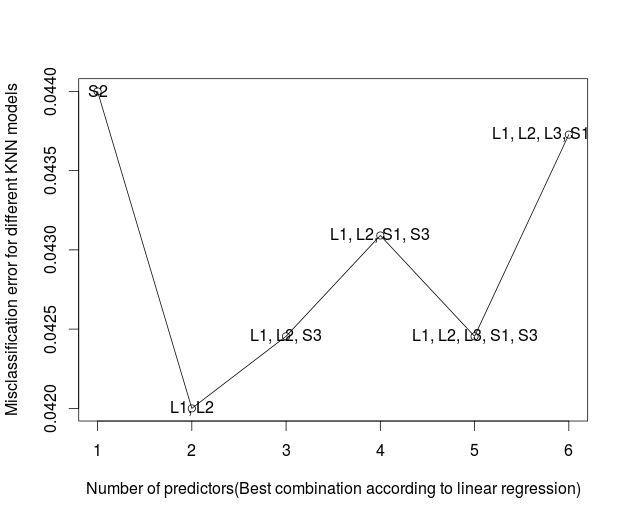
\includegraphics[scale=0.5]{img/error_knn.png}
\end{figure}
\end{itemize}

\section*{Conclusions}
\begin{itemize}
\item Marks of the first two languages(Typically Kannada and English) are the most accurate predictors of the NRC{\_}CLASS of a student.
\end{itemize}
